\section{The Wavelet Tree}
The Wavelet Tree is a binary balanced tree structure, that was invented by Grossi, Grupta and Vitter~\citeA{Grossi:2003:HET:644108.644250} in 2003. 
It has applications in many areas, from string processing to geometry, and can for instance be used to represent a sequence of elements, a reordering of elements or a grid of points. 
When~\citeA{Grossi:2003:HET:644108.644250} invented the Wavelet Tree, it was a milestone in compressed full-text indexing even though it is mentioned little in the paper.

\subsection{Constructing the Wavelet Tree}
\subsubsection{Informal Definition}
A Wavelet Tree stores a string in a binary tree of bitmaps, each bitmap indicating for each character in the corresponding string in which half of the alphabet it resides.

At the root node is stored a bitmap with the length of the input string, and each bit in this bitmap represents which half of the alphabet the character at the same position resides in.
At each node, the alphabet is split in half and the symbols in the left half are assigned bit value 0 in the bitmap and the symbols to the right are assigned bit value 1 so that there is a bit for each symbol in the string in the bitmap. 
The symbols of the string that has bit-value 0 are concatenated in the order they appear in the string and are passed as input string to the left sub-tree and the ones with bit value 1 are passed as input string to the right sub-tree.
Only the bitmaps are stored in each node.
The alphabet of the input string can be stored in the tree.
This process continues recursively in each sub tree until only one character is left in the alphabet of the input string of a sub tree.
The sub tree is then considered a leaf node and needs not store a bitmap.

An example of a Wavelet Tree can be seen in Figure~\ref{fig:WaveletTreeExample}.


\figureBegin
\Tree
%root
[.adsfadaadsfaads\\001100000110001 !\qsetw{5cm} 
	%left child
	[.adadaadaad\\0101001001 !\qsetw{5cm}
		%left -> left,right child 
		[.aaaaaa !\qsetw{5cm} ] [.dddd !\qsetw{5cm} ]] 
	%right child
	[.sfsfs\\10101 !\qsetw{5cm} 
		%right -> left,right child
		[.ff !\qsetw{5.3cm} ] [.sss !\qsetw{5.3cm} ]]] 
\caption{Wavelet Tree on string \textit{adsfadaadsfaads} with alphabet $\sigma = adfs$. Note that only the bitmaps are actually stored in the tree. The characters are annotations for ease of understanding.}	
\label{fig:WaveletTreeExample}
\figureEnd

\subsubsection{Formal Definition}
A Wavelet Tree for a sequence $S[1,n]$ over alphabet $[1 ... \sigma]$ can be described recursively over a sub-alphabet range $[a ... b] \subseteq [1 ... \sigma]$.
A Wavelet Tree over alphabet $[a ... b]$ (also called $\sigma$) is a binary balanced tree with $b - a + 1$ leaves. If $a = b$ then the Wavelet Tree is simply a leaf labelled $a$. 
Otherwise it has an internal root node $v_{root}$ that represents the string $S[1,n]$. 

Definition~\ref{def:SplittingTheString} defines more formally how the substrings of the input string passed to the left and right sub tree are constructed.


\vspace{0.5 cm}
\begin{mdframed}[nobreak, linecolor=lightgray, linewidth=2pt]
\begin{definition} Splitting the string. \\\\
Let $S_0[1,n_0] =$ subsequence of $S[1,n]$ formed by symbols $c \leq \sigma/2$.\\
Let $S_1[1,n_1] =$ subsequence of $S[1,n]$ formed by symbols $c > \sigma/2$.\\\\
Then the left child of $v_{root}$ is a Wavelet Tree for $S_0[1,n_0]$ over alphabet $[a ... \lfloor (a + b)/2 \rfloor]$ and right child of $v_{root}$ is a Wavelet Tree for $S_1[1,n_1]$ over alphabet $[1 + \lfloor (a + b)/2 \rfloor ... b]$.
\label{def:SplittingTheString}
\end{definition}
\end{mdframed}
\vspace{0.5 cm}


\subsubsection{Complexity}
The height of a filled Wavelet Tree is  $\lceil \log \sigma \rceil$ and it has $\sigma$ leaves and $\sigma - 1$ internal nodes. 
At each level in the tree at most \textit{n} bits are stored in the bitmaps in total.
If some characters of the alphabet do not occur in the input string, the sub trees of the Wavelet tree corresponding to those missing characters may be omitted depending on implementation.
$n \lceil \log \sigma \rceil$ is an upper bound to the total number of bits that the Wavelet Tree stores in its bitmaps.
The Wavelet Tree can theoretically be constructed in $O(n \log \sigma)$ time as the entire inputs string must be processed once fully for each layer of nodes, the string and the work split out among the nodes of that layer.


\subsubsection{Pseudocode}
\label{sec:nodeconstruction}
The Wavelet Tree construction algorithm is recursively defined, calling itself to construct the left and right sub-tree from the root node and down. At each recursion the algorithm splits the given alphabet in two halves and traverses the given string putting each character into a left or right partition based on whether the character was in the left or right half of the alphabet.

\begin{algorithm}
\caption{Construction of nodes in the Wavelet Tree}
\label{alg:ConstructNode}
\begin{algorithmic}
\Function {ConstructNode} {$String, Alphabet$}
\If{$Alphabet.Size() = 1$ or $String.Length() = 0$}
	\State \Return
\EndIf
\State Split $Alphabet$ into $LeftAlphabet$ and $RightAlphabet$
\State $Split \gets$ middle character in $Alphabet$
\ForAll {$Character$ in $String$}
	\If {$Character < Split$}
		\State $LeftString.Append(Character)$
		\State $Bitmap.Append(0)$
	\Else
		\State $RightString.Append(Character)$
		\State $Bitmap.Append(1)$
	\EndIf
\EndFor
\State $LeftNode \gets$ \Call {ConstructNode} {$LeftAlphabet, LeftString$}
\State $RightNode \gets$ \Call {ConstructNode} {$RightAlphabet, RightString$}
\EndFunction

\State \Call {ConstructNode} {InputString, InputAlphabet}
\end{algorithmic}
\end{algorithm}

\subsection{Rank Query}
\label{sec:rankDescription}

\begin{algorithm}
\caption{Rank}
\label{alg:rank}
\begin{algorithmic} 
\Function {Rank} {$Character, Position$}
\If{$Self.IsLeaf()$}
\State \Return $Position$
\EndIf
\State $CharBit \gets$ bit representing $Character$ in bitmap of current node
\State $Occurrence \gets$ \Call {BinaryRank} {$CharBit, Position, BitMap$}
\If{$CharBit = 1$}
	\State $Rank \gets$ RightChildNode.\Call {Rank} {$CharBit, Occurrence$}
\Else
	\State $Rank \gets$ LeftChildNode.\Call {Rank} {$CharBit, Occurrence$}
\EndIf
\State \Return $Rank$ 
\EndFunction
\State RootNode.\Call {Rank} {$Character, Position$}
\end{algorithmic}
\end{algorithm}

Rank counts the number of occurrences of the specified character up to and including the specified position. 
It starts from the root of the Wavelet Tree and moves down through the tree until it hits the leaf of the input character.
In each level of the tree \textproc{BinaryRank} is calculated for the character. 
The result of \textproc{BinaryRank} is used as the position parameter for the next recursive call to rank.
When the leaf of the input symbol is reached, the position returned from the previous call to \textproc{BinaryRank} is already the rank of the input symbol up to the original input position.
Intuitively this makes sense because leaf nodes correspond to only one character and the rank of a character up to a position in a string containing only that character is the same as the position.
Figure~\ref{fig:RankDrawing} shows an example of how this concept works.

Whether the query uses the left or right child in the recursive call is decided by what the symbol in represented as in the bitmap of the current node.
This is computed by finding which character corresponds to the middle of the alphabet for the current node, the "split character", and then check whether the queried-for symbol is lexicographically less than or equal to the split character. 
If this is the case the input symbol is represented by 0 since it would be in the alphabet of the left child.
If it is not the case then the input symbol is represented as 1.

C++ is used for our implementation and the object-oriented paradigm is utilized and therefore \textproc{Rank($Character, Position$)} is defined on each node, and so, in the pseudo-code, it is called on the root node and the right and left child nodes instead of specifying the node as a parameter to the \textproc{Rank} function, as one would have done it in plain C.

\begin{figure}
\center 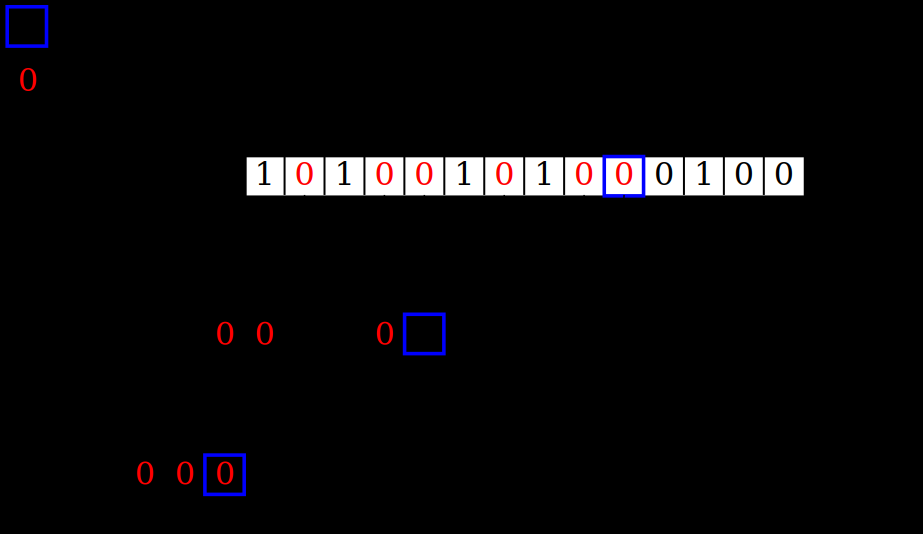
\includegraphics[width=0.66\textwidth]{RankDrawing}
\caption{Rank: This figure shows why the rank algorithm works. The number of occurrences of 0s or 1s, depending on how the character is represented, are used as the position in the next level. 
When the leaf is reached the position corresponds to the number of occurrences.}
\label{fig:RankDrawing}
\end{figure}

\subsubsection{Binary Rank} 
\label{sec:TheoryBinaryRank}
\begin{algorithm}
\caption{BinaryRank}
\label{alg:binaryrank}
\begin{algorithmic}
\Function {BinaryRank} {$Position, Bitmap$}
	\State $i \gets 0$
	\State $rankValue \gets 0$
	\For{$bit$ in $Bitmap$}
		\If{$i > Position$}
			\State \Return $rankValue$
		\EndIf
		\If{$bit = 1$}
			\State $rankValue \gets rankValue + 1$
		\EndIf
		\State $i \gets i + 1$
	\EndFor
\EndFunction
\end{algorithmic}
\end{algorithm}

\textproc{BinaryRank} [Algorithm~\ref{alg:binaryrank}] returns the number of 1s until a given position.
It does so by looping the bitmap until the specified position and counts the number of 1s along the way.
When the position is reached the number of 1s is returned.
This takes $O(n)$ time.
In Section~\ref{sec:popcountBinaryRank} we describe how to improve the practical running time.


\subsection{Select query}
\label{sec:selectDescription}
\begin{algorithm}
\caption{Select}
\label{alg:select}
\begin{algorithmic} 
\Function {Select} {$Character, Occurrence$}
\State $Leaf \gets GetLeaf(Character)$
\If{$Leaf$ is $RightChild$}
	\State $CharBit \gets 1$
\Else
	\State $CharBit \gets 0$
\EndIf
\State \Return $Leaf.Parent.$\textproc{SelectRec}$(CharBit, Occurrence)$
\EndFunction

\vspace{1cm}

\Function {SelectRec} {$CharBit, Occurrence$}
\If{$CurrentNode$ is $root$}
	\State \Return \textproc{BinarySelect}$(CharBit, Occurrence)$
\EndIf
\State $Position \gets $\textproc{BinarySelect}$(CharBit, Occurrence)$
\If{$CurrentNode$ is $RightChild$}
	\State $CharBit \gets 1$
\Else
	\State $CharBit \gets 0$
\EndIf
\State \Return $Parent.$\textproc{SelectRec}$(CharBit, Position)$
\EndFunction

\vspace{1cm}

\Function {GetLeaf} {$Character$}
\If{Self.isLeaf}
	\State \Return Self
\EndIf
\State $CharBit \gets character >$ middle character of alphabet
\If{$CharBit = 1$}
	\State \Return RightChild.GetLeaf($Character$)
\ElsIf{$CharBit = 0$}
	\State \Return LeftChild.GetLeaf($Character$)
\EndIf
\EndFunction
\end{algorithmic}
\end{algorithm}

\begin{figure}
\center 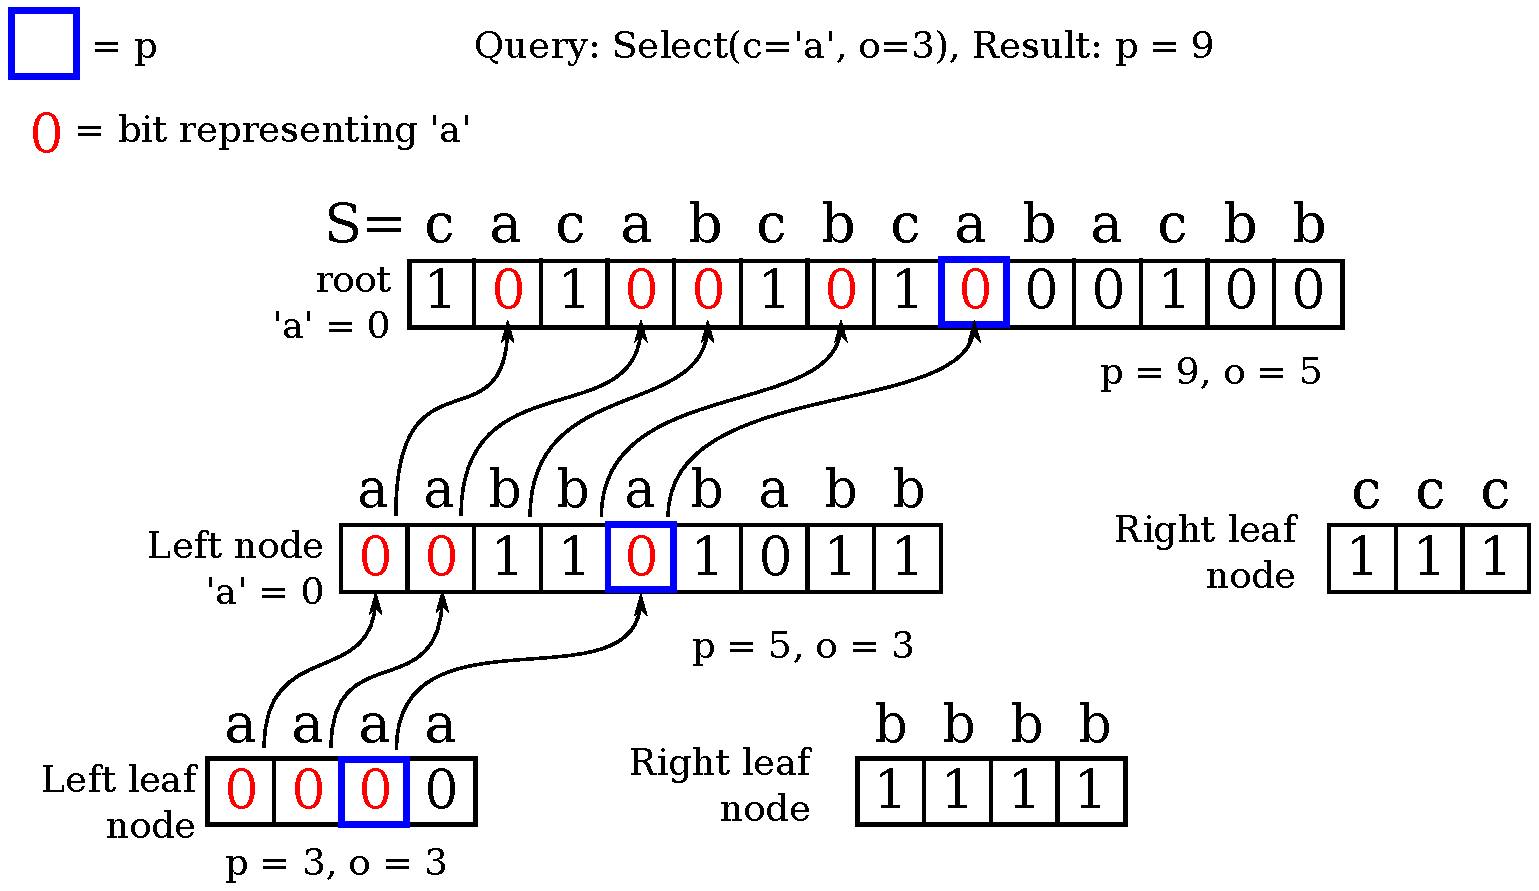
\includegraphics[width=0.66\textwidth]{SelectDrawing}
\caption{Select: This figure shows why the select algorithm works. 
In this example we want to find the position of the 3rd occurrence of \textit{a} which is represented as 0 in the leaf.
Starting from the leaf, the position of the specified occurrence is used as the occurrence to find the position of in the parent. 
In each level the algorithm looks for either 0 or 1 based on how \textit{a} is represented in the specific node.
In the root the algorithm looks for the position of the 5th occurrence of 0 which is 9 and corresponds to the position of the 3rd \textit{a}.
The process terminates when the root is reached.}
\label{fig:SelectDrawing}
\end{figure}

\textproc{Select} queries searches the Wavelet Tree for the position of the $i^{th}$ occurrence of the specified character.
It starts from the leaf of the character and walks up through parent nodes to the root of the tree, which means it is necessary to know the leaf of the character. 
This is accomplished using the \textproc{GetLeaf} method, which works by recursing down the tree from the root and choosing the right or left path based on whether the queried-for character is represented as a 0 or a 1 in the bitmap of the current node.
The recursion stops when the leaf of the character is found.
After having found the leaf the \textproc{Select} function can then compute which bit represents all the characters in the leaf node, called \textit{CharBit}, by knowing whether it is a right- or a left-child of its parent node.

\textproc{SelectRec} is then called on the parent of the leaf which recursively traverses up the tree towards the root to find the position of the specified occurrence of the input character.
It does so by calling \textproc{BinarySelect} which returns the position of the specified occurrence of the \textit{CharBit} in the bitmap of the current node. 
This position is then used as the occurrence to find the position of in the next recursive call.
When the root is reached the result of \textproc{BinarySelect} is the position of the specified occurrence of the character in the original input string and can be returned as such.

Select queries are performed in collaboration by the \textproc{Select} and \textproc{SelectRec} functions because using two functions instead of one saves us a check for whether the current node is a leaf or not at each recursive call and since we start out in a leaf and will never meet one again that check would only be true once during the execution.

Figuring out the \textit{CharBit} is a lot simpler for \textproc{Select} than for \textproc{Rank} since we query bottom-up and can just check whether the current node is a left child or a right child. 
In \textproc{Rank} one needs to calculate the split character and then check whether the input character is before or after it in the alphabet in every recursive step.

An example of how the intuition behind why \textproc{Select} works is shown in Figure~\ref{fig:SelectDrawing}.
In the example the algorithm looks for the position of the 3rd \textit{a}.
It starts in the leaf of \textit{a} and finds that he position of the 3rd \textit{a} is 3. 
This position is then used in the parent as the occurrence to find the position of. 
The new position becomes 5.
In the root the algorithm then looks for the position of the 5th occurrence which is 9 and corresponds to the position of the 3rd \textit{a}.
I each level the algorithm looks for either 0 or 1 based on how \textit{a} is represented in that level.

\subsubsection{Binary Select}
\label{sec:binarySelectDescription}
\begin{algorithm}
\caption{BinarySelect}
\label{alg:binaryselect}
\begin{algorithmic}
\Function {BinarySelect} {$Occourance, Bitmap, BitToCount$}
\State $Occ \gets 0$
\For{$bit$ in $Bitmap$}
	\If{$bit = BitToCount$}
		\If{$Occ = Occourance$}
		\State \Return position of $bit$ in $Bitmap$
	\EndIf
	\State $Occ \gets Occ + 1$
	\EndIf
\EndFor
\EndFunction
\end{algorithmic}
\end{algorithm}

\textproc{BinarySelect} returns the position of the \textit{i}th occurrence of 1 or 0 (\textit{CharBit}) in a bitset. 
It does so by looping through the bitmap and when \textit{i} occurrences of either 1 or 0 (depending on whether the current node is a left child or a right child) has been seen then the position of the last bit that was seen is returned.
\textproc{BinarySelect} takes O(n) time because the length of a bitmap is at most the length of the original input string.
In Section~\ref{sec:ImplBinarySelect} we describe how to improve the practical running time of \textproc{BinarySelect}.

